
\documentclass[12pt]{article}
\usepackage[a4paper, margin=.30in]{geometry}
\usepackage{graphicx ,
            wrapfig,
            xcolor, 
            enumerate,
            amsmath,
			fontenc,
			tcolorbox,circuitikz,tikz,bm
            }
			\usepackage{pgfplots}
\pgfplotsset{compat=newest}
\usepgfplotslibrary{fillbetween}
%\usepackage{scalerel}
%\usepackage{pict2e}
%\usepackage{tkz-euclide}
%\usetikzlibrary{calc}
%\usetikzlibrary{patterns,arrows.meta}
%\usetikzlibrary{shadows}
%\usetikzlibrary{external}

%%pgfplots
\usepackage{pgfplots}
%\pgfplotsset{compat=newest}
%\usepgfplotslibrary{statistics}
%\usepgfplotslibrary{fillbetween}

\newcommand\headerMe[2]{\noindent{}#1\hfill#2}
\renewcommand{\thesection}{\Roman{section}}

\author{Zakaria HAOUZAN}
\date{\today}

\begin{document}
% headers --------------
\headerMe{Matière : Physique-Chimie}{Professeur : Zakaria HAOUZAN}\\
\headerMe{Unité : Mécanique }{Établissement : Lycée SKHOR qualifiant}\\
\headerMe{Niveau : 2BAC-SM-PC}{Heure : 7H}\\

% ------Content ________
\begin{center}

    \Large{Leçon $N^{\circ} 12 $: \color{red} Les mouvement plans}
\end{center}

%\begin{wrapfigure}[10]{r}{0.5\textwidth}
%    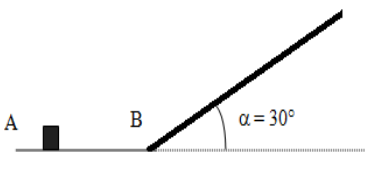
\includegraphics[width=0.5\textwidth]{./img/img00.png}
%\end{wrapfigure}


\section{Introduction }
Dans ce chapitre, nous étudierons différents types de mouvements plans, c'est-à-dire des mouvements qui se produisent dans un plan à deux dimensions. Nous analyserons quatre situations fondamentales :

\begin{itemize}
  \item Le mouvement d'un solide sur un plan horizontal et sur un plan incliné
  \item Le mouvement d'un projectile dans le champ de pesanteur uniforme
  \item Le mouvement d'une particule chargée dans un champ électrique uniforme
  \item Le mouvement d'une particule chargée dans un champ magnétique uniforme
\end{itemize}

\section{Mouvement d'un solide sur un plan horizontal et sur un plan incliné:(Rappel)}
\section{Le mouvement d'un projectile dans le champ de pesanteur:}

\subsection{Étude Expérimentale(Trajectoire du projectile) : }


Au début la bille est maintenue par électroaimant puis lâchée du haut d’un rail ,elle roule le long du rail et elle le
quitte avec une vitesse initiale horizontale puis elle tombe sur une plaque horizontale.
En faisant varier la position de la plaque et en indiquant chaque fois sa position de chute de la bille, on obtient la
trajetoire de son mouvement: c'est une trajetoire parabolique.

\begin{itemize}
  \item Quel est le mouvement de la bille dans le champ de pesanteur ?
  \item Comment varie le vecteur vitesse et le vecteur accélération ?
  \item Comparer le vecteur accélération et g ?
\end{itemize}
\subsection{Etude du mouvement du projectile :}

Un projectile de masse m est lancé d'un point O à l'instant $t=0$ avec une vitesse $\vec{v_0}$ qui fait un angle $\alpha$ avec l'horizontale.

On considère un repère $(O, \vec{i}, \vec{j})$ confondu avec le plan du mouvement du projectile et qu'on suppose galiléen.

\begin{itemize}
	\item Le système étudié :{le projectile}
	\item Bilan des forces: le projectile est soumis uniquement à l'action de son poids :
		(Le projectile a une grande densité ,donc la poussée d'Archimède et les forces de frottement fluides sont négligeable)
	\item Les conditions initiales à $t=0$ ,$x_0=0$ et $y_0=0$
	\item Les coordonées du vecteur vitesse initiale sont : 
		$\begin{cases} v_{0x} = v_0.cos(\alpha)\\v_{0y} = v_0.sin(\alpha)
\end{cases}$
	\item En appliquant la 2ème loi de Newton : $\sum \vec{F}=m\vec{a_G}$ donc $\vec{P} = m.\vec{a_G}$ (1)

	\item  Par projection de la relation (1) dans le repère (O,x,y): 
$\begin{cases}P_x = m.a_x\\P_y = m.a_y\end{cases}$
 alors $\begin{cases}0 = m.a_x\\-P = m.a_y\end{cases}$
 donc $\begin{cases}a_x = 0\\a_y = -g\end{cases}$
 avec $\begin{cases}\frac{dv_x}{dt} = 0\\\frac{dv_y}{dt} = -g\end{cases}$  $\rightarrow$ 
  $\begin{cases}v_x = C\\v_y = -gt+C'\end{cases}$

\item On détermine les constantes C et C' d'après les conditions initiales : à t=0 : 

	$\begin{cases} v_{0x} = v_0.cos(\alpha)\\v_{0y} = v_0.sin(\alpha) \end{cases}  \Rightarrow$ 	
	$\begin{cases} v_{x} = v_0.cos(\alpha)\\v_{y} = -g.t +v_0.sin(\alpha) \end{cases} $
	d’où  $\begin{cases} \frac{dx}{dt} = v_0.cos(\alpha)\\\frac{dy}{dt} = -gt+v_0.sin(\alpha) \end{cases}$ 	

	donc  : $\begin{cases} x = v_0.cos(\alpha).t + K\\y = \frac{-1}{2}.gt^2 + v_0.sin(\alpha).t + K' \end{cases}$ 	

\item On détermine les constantes K et K' d'après les conditions initiales : à t=0 , xo=0 et yo=0 donc :K=0 et K'=0. 
	 
	Et on obtient les équations horaires du mouvement du projectile : $\begin{cases} x = v_0.cos(\alpha).t + K\\y = \frac{-1}{2}.gt^2 + v_0.sin(\alpha).t + K' \end{cases}$


	\item On obtient l'équation de la trajectoire en éliminant t entre x et y.

	On a $t =  \frac{x}{v_0.cos(\alpha)}$ en remplaçant dans y : $y = -\frac{g}{2.v_0^2.cos(\alpha)^2}.x^2 +xtan(\alpha)$

\item Le sommet S de la trajectoire : c'est le plus haut point atteint par le projectile au cours de son mouvement.
	\begin{itemize}
		\item Au sommet de la trajectoire on a $v_y = 0$ donc $t=\frac{v_0.sin(\alpha)}{g}$
		\item Et en remplaçant dans x et y on obtient les coordonnées du sommet S de la trajectoire du projectile. $y_s =\frac{v_0^2.sin(\alpha)^2}{2g}$ et $x_s = \frac{v_0^2.sin(2.\alpha)}{2g}$
		\item avec: $sin(2\alpha) =2.sin(\alpha) . cos(\alpha)$
	\end{itemize}

\item La portée :c'est la distance OP qui sépare le point de lancement du projectile et le point de sa tombée sur ox. Au point P on a $y_p = 0 \Rightarrow 0 = -\frac{g}{2.v_0^2.cos(\alpha)^2}.x^2 +xtan(\alpha)$alors : $\begin{cases} x_p = 0 \\ x_p = \frac{x^2.sin(2\alpha)}{g}\end{cases}$
\item Remarque: La plus grande portée correspond à $sin(2.\alpha) =1$ donc $\alpha = \frac{\pi}{4}$

\end{itemize}


\section{Mouvement d'une particule chargée dans un champ magnétique
uniforme.}
\subsection{Le champ magnétique uniforme.}

\begin{wrapfigure}{r}{0.2\textwidth}
	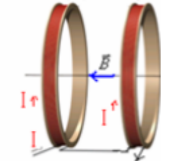
\includegraphics[width=0.2\textwidth]{./Helmholtz.png}
\end{wrapfigure}
Un champ magnétique est dit uniforme s'il est constant en direction, en sens et en valeur .

Exemple : Le champ magnétique est uniforme entre les bobines d'Helmholtz parcourues par un courant électrique.

L'unité de l'intensité du champ magnétique est le tesla (T). 

Remarque: Si le vecteur $\vec{B}$ est perpendiculaire au plan de la feuille et dirigée vers l'avant on le Représente par $\bigodot$

Si le vecteur $\vec{B}$ est perpendiculaire au plan de la feuille et dirigée vers l'arrière on le Représente par $\bigoplus$

\subsection{Déviation d'unr particule chargée dans un champ magnétique uniforme : }


\subsubsection{Expérience : }
On utilise un tube de crookes (qui contient un canon d'électrons permetant d'obtenir un faisceau d'électrons ayant la même
vitesse) à l'intérieur duquel il y'a un champ magnétique uniforme entre deux bobines d'Helmholtz parcourues par un courant
électrique.

On constate expérimentalement que : 

\begin{enumerate}

 \item Si la vitesse des électrons $\vec{v_0}$ est parallèle à $\vec{B}$ , le faisceau d'électrons ne subit pas de déviation.

 \item Si la vitesse des électrons $\vec{v_0}$ est perpendiculaire à $\vec{B}$ , le faisceau d'électrons dévie et sa transitoire est devient circulaire . 
\end{enumerate}

\subsubsection{Interprétation: }
La déviation du faisceau d'électron est du à l'existence d'une force magnétique qui s'exerce sur toute particule chargée
et en mouvement dans un champ magnétique uniforme qu'on appelle : force magnétique ou force de Lorentz.

\section{La force magnétique : }
Toute particule chargée de vitesse $\vec{v}$
est soumise dans un champ magnétique uniforme à une force magnétique appelée force de Lorentz donnée par la relation suivante:
$$\vec{F} = q.\vec{v} \wedge \vec{B} $$

le symbole: $\wedge$ signifie produit vectoriel.

Caractéristiques de la force magnétique:
\begin{itemize}
	\item La direction : la force magnétique $\vec{F}$ est perpendiculaire au plan $(\vec{B}, \vec{v})$.
	\item Le sens : il est donné par la règle de la main droite suivante:

		En plaçant la main droite tendue de sorte les doigts soient dirigés dans le sens du produit $q.\vec{v}$ et la paume de la main soit dirigée dans le sens de $\vec{B}$,le pouce tendu indique le sens de la force magnétique . 
		\begin{center}
			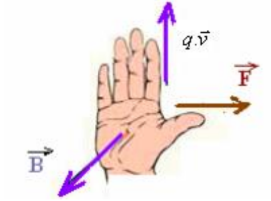
\includegraphics[width=0.2\textwidth]{./hand.png}
			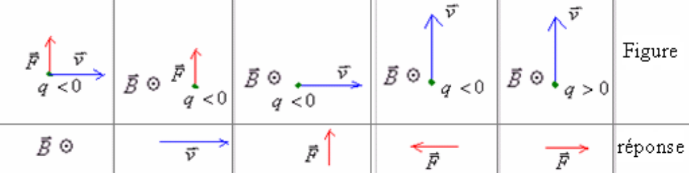
\includegraphics[width=0.5\textwidth]{./exemple.png}
		\end{center}
		Remarque: Si la charge $q>0$ le produit $q.\vec{v}$ a le même sens que le vecteur vitesse $\vec{v}$.

 Si la charge $q < 0$ le produit $q.\vec{v}$ a le sens contraire que celui du  vecteur vitesse $\vec{v}$.


 Exemples : compléter les figures suivantes: 

\item L'intensité $F = |q|.v.B.\sin(\vec{B},\vec{v})$

\end{itemize}
\subsection{Etude du mouvement d'une particule chargée dans un champ magnétique
uniforme.}

\subsubsection{Montrons que le mouvement de l'électron dans le champ magnétique est uniforme:}
L'électron dans le champ magnétique est soumis à l'action de la force magnétique $\vec{F} = q.\vec{v} \wedge \vec{B}$, cette force de Loreentz est
toujours perpendiculaire au vecteur vitesse $\vec{v}$ donc le produit scalaire $\vec{F}.\vec{v} = 0$ 

par conséquence la puissance de la force magnétique est nulle : $P = \vec{F}.\vec{v} = 0$ donc son travail est nul $W(F) = 0$.

En appliquant le théorème de l'énergie cinétique : $\Delta{E_c} = W(F) = 0$ donc $E_ci = E_cf$

Donc sa vitesse v= Cte ., donc l'action du champ magnétique ne modifie pas l'énergie cinétique de la particule
\subsubsection{Montrons que le mouvement de l'électron dans le champ magnétique est plan:}
la vitesse de l'électron $v=Constante$

son accélération tangentielle $a_t = \frac{dv}{dt} = 0$ donc l'accélération de l'électron est normale.

On a $\vec{F} = q.\vec{v} \wedge \vec{B}$ la force magnétique $\vec{F}$
qui perpendiculaire au plan $(\vec{B}, \vec{v})$ est elle aussi normale.

Donc le mouvement de l'électron est plan , il se fait dans un plan perpendiculaire au vecteur champ magnétique.

\subsubsection{Montrons que le mouvement de l'électron dans le champ magnétique est circulaire: }
Dans le repère de frenet le vecteur accélération $a = a_N.\vec{n} + a_t.\vec{u}$

or V = Cst $\rightarrow$ $a_t = \frac{dv}{dt} = 0$

En appliquant la deuxième loi de Newton $\vec{F} = m.a_G\rightarrow  q.\vec{v} \wedge \vec{B} = m.\vec{a_G}$

Dans le repère de Frenet : $\vec{a_G}$ : $\begin{cases}a_t = \frac{dv}{dt} = 0\\ a_n = \frac{v^2}{R}\end{cases}$
 Donc $a = a_n$ l'accélération est normale.

 En projectant la relation (1) sur la normale $|q|.v.B = m.\frac{v^2}{R}$

 Le rayon est constant donc le mouvement est circulaire:  $R = \frac{m.v}{|q|.B}$


 \subsubsection{La Déviation magnétique : }
On fait pénetrer un faisceau d'électron dans une région de l'espace de largeur $l$
dans laquelle règne un champ magnétique $\vec{B}$

uniforme avec une vitesse $\vec{v_0}$ , le faisceau d’électrons est soumis à l'action de la force magnétique et son mouvement

devient circulaire de rayon :$R = \frac{m.v}{|q|.B}$
dans le champ magnétque.

Les électron du faisceau quittent le champ magnétique au point S et prennent un mouvement rectiligne uniforme

jusqu'à ce qu'ils rencontrent l'écran au point P.

Le faisceau d'électron rencontre l'écran au point O'.

On appelle déviation magnétique la distance $D_m$=O'P

On a dans le triangle rectangle $(HM'I)$ : $\sin{\alpha} = \frac{l}{R}$

et dans le triangle rectangle $JPO$ : $\tan{\alpha} = \frac{D_m}{D}$

Dans les appareils utilisés on a généralement des angles $\alpha$ petits , on a alors $\sin{\alpha} \equiv \tan{\alpha} $

		\begin{center}
			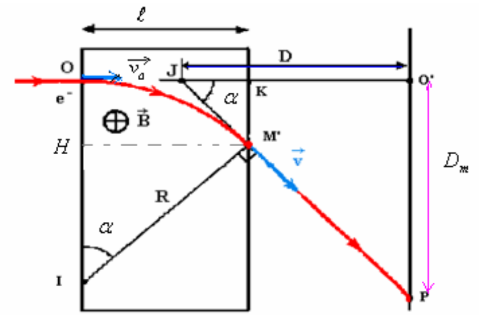
\includegraphics[width=0.5\textwidth]{./deviation.png}
		\end{center}


$$\frac{D_m}{D} = \frac{l}{R}$$ avec $R = \frac{m.v_0}{|q|.B}$  donc la déviation magnétique $$D_m = \frac{l.D.|q|.B}{m.v_0}$$

\section{Applications : Le spectromètre de masse : }
Le spectromètre de masse est un appareil qui permet de séparer des ions ayant des masses et des charges différentes
(comme les isotopes )en utilisant les actions d'un champ magnétique et d'un champ électrique, il se compose de:

\textbf{Une chambre d'ionisation }: à partir de laquelle partent les ions avec une vitesse nulle.

\textbf{Une chambre d'accélération:} dans laquelle on accélère les ions par un champ électrique uniforme et les ions la quitte
. avec une vitesse $\vec{v}$

\textbf{Une chambre de séparation}: dans laquelle on sépare les ions en utilisant un champ magnétique uniforme $\vec{B} \perp \vec{v} $  et dans laquelle les ions décrivent une trajectoire demi-circulaire.

	\begin{center}
			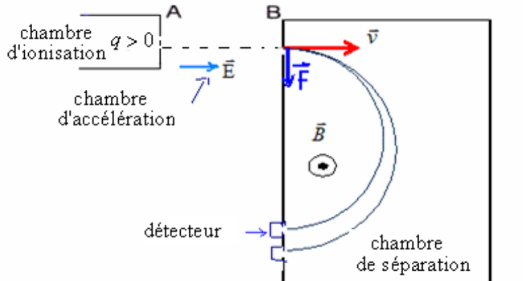
\includegraphics[width=0.5\textwidth]{./chambre.png}
		\end{center}

Les ions sont accélérés par un champ électrique uniforme dans la chambre d'accélération :
En appliquant le théorème de l'énergie cinétique entre A et B :

 $\Delta{{E_c}_{A\rightarrow B}} = {{W(F)}_{A \rightarrow B}}$

 $\frac{1}{2}.mv^2 - 0 = qU_{AB}$ donc $v = \sqrt{\frac{2qU_{AB}}{m}}$

 Or les ions ont des masses différentes, ils pénètrent dans la chambre de séparation par des vitesses différentes.

 Lorsque l'ion qui pénètre dans la chambre de séparation avec une vitesse $\vec{v} \perp \vec{B}$ il sera soumis à l'action de la force magnétique $\vec{F} = q.\vec{v} \wedge \vec{B}$ et aura un mouvement circulaire de rayon $R = \vec{m.v_0}{|q|.B}$

 Chaque ion décrira un demi cercle de diamètre $D = 2R = 2.\frac{m.v_0}{|q|.B}$

 Or le rayon dépend de la masse, chaque isotope aura un cercle différent de celui des autres, ce qui permettra de
séparer les isotopes les uns des autres.

\subsection{Le cyclotron:}
Le cyclotron est un accélérateur de particules ; il se compose de deux boites sous forme de demi cylindre appelées :
des "dees" posées dans un champ magnétique uniforme et entre les boites existe un oscillateur qui produit un champ
électrique uniforme et alternatif de période T égale à la demi période de rotation de la particule dans sa trajectoire
circulaire et de cette façon la particule est accélérée chaque fois qu'elle pénètre dans le champ électrique et finalement
la particule quitte le cyclotron avec une grande vitesse.


 %wfg---------------------------------------------------------------sf 
%\begin{center}
   %\begin{tabular}{ |c|c|c|c|c|c|c| }
      %\hline
      %km & hm & dam & \bf{m} & dm & cm & mm \\
      %\hline
        %&   &    &  &   &   & \\
%\hline
%\end{tabular}
%On place un seul nombre dans chaque case.
%\end{center}
%\begin{center}
   %\begin{tabular}{ |c|c|c|c|c|c|c| }
      %\hline
      %$km^2$ & $hm^2$ & $dam^2$ & \bf{$m^2$} & $dm^2$ & $cm^2$ & $mm^2$ \\
      %\hline
        %&   &    &  &   &   & \\
%\hline
%\end{tabular}
%\end{center}


\end{document}

